\subsection*{ГЛ11 7}
\begin{figure}[h]
	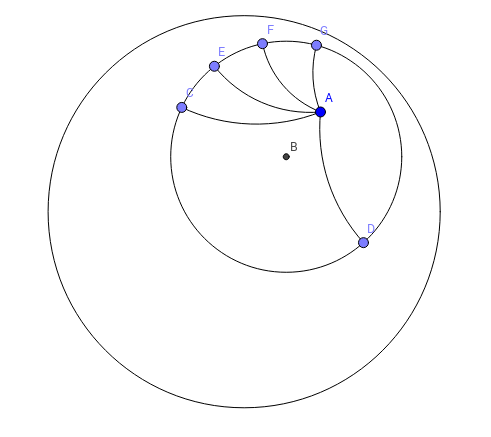
\includegraphics[width=0.5\linewidth]{pic8}
\end{figure}
зададим перспективную систему координат
\begin{gather*}
	\begin{cases}
		S = \alpha_1 A_1 + \alpha_2 A_2\\
		S = \beta_1 B_1 + \beta_2 B_2\\
		S = \gamma_1 C_1 + \gamma_2 C_2
	\end{cases}
	\\
	\alpha_1 A_1 - \beta_1 B_1 = -\alpha_2 A_2 + \beta_2 B_2
\end{gather*}
Так как 
\begin{gather*}
	A_1B_1 \cap A_2B_2 = P
\end{gather*}
То
\begin{gather*}
	P = \alpha_1A_1 - \beta_1 B_1 = -\alpha_2 A_2 + \beta_2 B_2
\end{gather*}
Аналогично
\begin{gather*}
	Q = \beta_1 B_1 - \gamma_1 C_1 = -\beta_2 B_2 + \gamma_2 C_2\\
	R = \gamma_1 C_1 - \alpha_1 A_1 = -\gamma_2 C_2 + \alpha_2 A_2\\
	\\
	P+Q+R = 0\\
	P = -Q-R
\end{gather*}
Следовательно $P,Q,R$ принадлежат одной прямой\\
Если же $A_1A_2 \cap B_1B_2 \cap C_1C_2 \ne S$ то $P,Q,R \ne 1$ откуда следует что $P,Q,R$ не коллинеарны
		 
	